
\documentclass[11pt]{article}
\PassOptionsToPackage{svgnames}{xcolor}
\usepackage{graphicx} % Required for inserting images
\usepackage[utf8]{inputenc}
\usepackage[margin=1in]{geometry}
\usepackage{enumerate, fancyhdr, color, verbatim, setspace, multirow, multicol,subcaption, booktabs, caption, amsfonts}
\usepackage{rotating}
\usepackage{amsmath}
\usepackage{amsthm}
\usepackage{cancel}
\usepackage{listings}
\usepackage{algorithm}
\usepackage{algpseudocode}
\numberwithin{equation}{section}
\newtheorem{definition}{Definition}[subsection]
\newtheorem{theorem}{Theorem}[subsection]
\newtheorem{corollary}{Corollary}[subsection]
\newcommand{\E}{\mathbb{E}}
\newcommand{\Var}{\mathbb{V}}


\usepackage{colortbl}
\usepackage{tikz}
\usetikzlibrary{matrix, positioning, shadings, shadows}
\usepackage{pgfplots}
\pgfplotsset{compat=1.18}
\usepackage[shortlabels]{enumitem}
% \usepackage[symbol]{footmisc}
\usepackage{multirow}
\usepackage{multicol}
% Creates the header and footer. You can adjust the look and feel of these here.
\usepackage{hyperref}
\hypersetup{
    colorlinks,
    citecolor=black,
    filecolor=black,
    linkcolor=blue,
    urlcolor=blue
}
\newcommand{\bp}{\mathbb{P}}

\definecolor{lightgray}{RGB}{230, 230, 230}
\definecolor{lightgrey}{RGB}{200, 200, 200}

\usepackage{tcolorbox}
\newenvironment{myblock}[1]{%
    \tcolorbox[beamer,%
    noparskip,breakable,
    colback=lightgray,colframe=black,%
    colbacklower=lightgrey,%
    title=#1]}%
    {\endtcolorbox}

\tcbuselibrary{skins,breakable}


\renewcommand{\headrulewidth}{0.2pt} %Creates a horizontal line underneath the header
\setlength{\headheight}{15pt} %Sets enough space for the header
% \renewcommand{\theenumi}{\alph{enumi}}
\onehalfspacing

\usepackage{chngcntr}
\counterwithin{figure}{section}

\DeclareMathOperator*{\argmin}{arg\,min}
\DeclareMathOperator*{\argmax}{arg\,max}

\usepackage[backend=biber, style=authoryear, maxcitenames=2, maxbibnames=9]{biblatex}
\DeclareDelimFormat{nameyeardelim}{\addcomma\space}
\addbibresource{references.bib}

\setcounter{tocdepth}{2}

\title{MGTECON 603 - Problem Set 3\\ \small{(Instructor: Guido Imbens)}}
\author{Wooyong Park\\ {\small Collaborators: Cem Kozanoglu, Roberto Gonzalez Tellez, Hanniel Ho, Aileen Wu}}
\date{\today}

\begin{document}


\maketitle

\section{Part I}

\subsection*{Descriptive Statistics}

The summary statistics of the data are shown in tables \ref{tab:summary_stats}, \ref{tab:summary_stats(control_group)}, and \ref{tab:summary_stats(treated_group)} in the appendix.

The histogram of the outcome variable \verb|earnings1yr| (Figure \ref{fig:hist_earnings1yr}) and \verb|earnings4yr| (Figure \ref{fig:hist_earnings4yr}) display a heavily zero-inflated distribution, and overall we have more treated units than control units.

\begin{figure}[h]
    \centering
    \begin{subfigure}{0.48\textwidth}
        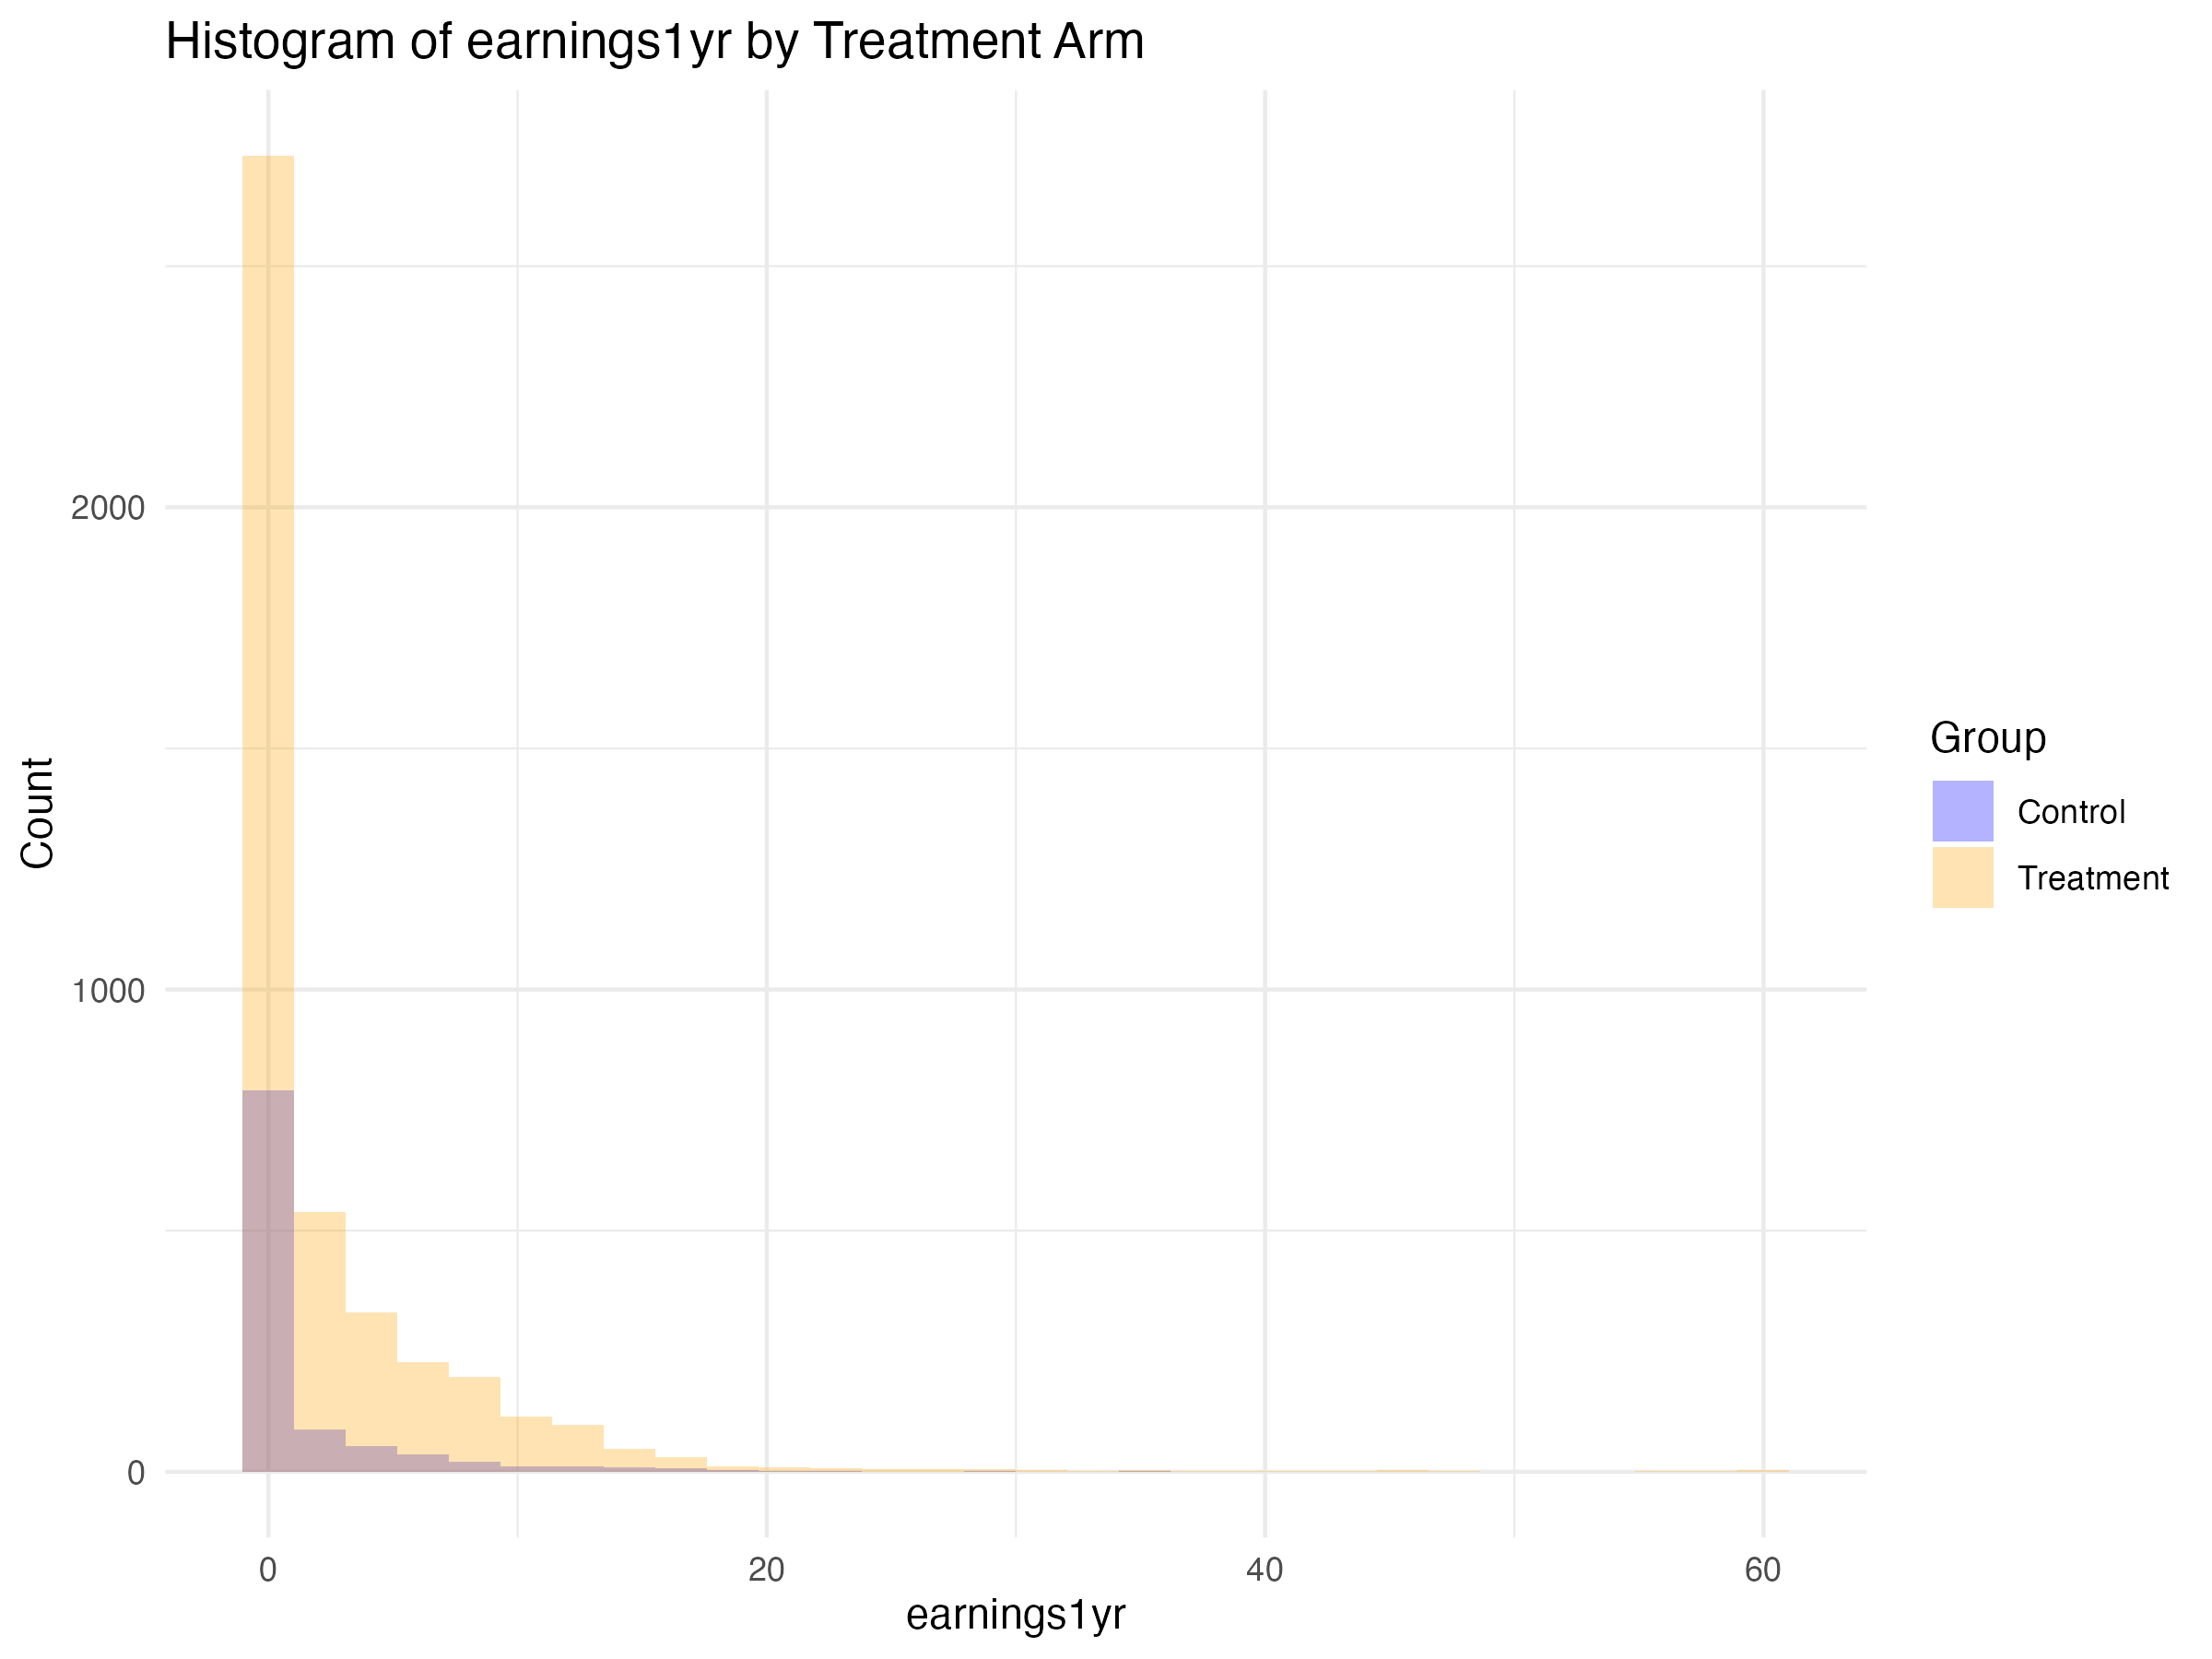
\includegraphics[width=0.8\textwidth]{output/histogram_earnings1yr_by_treatment_arm.png}
        \caption{\label{fig:hist_earnings1yr}Earnings one year after treatment}
    \end{subfigure}
    \begin{subfigure}{0.48\textwidth}
        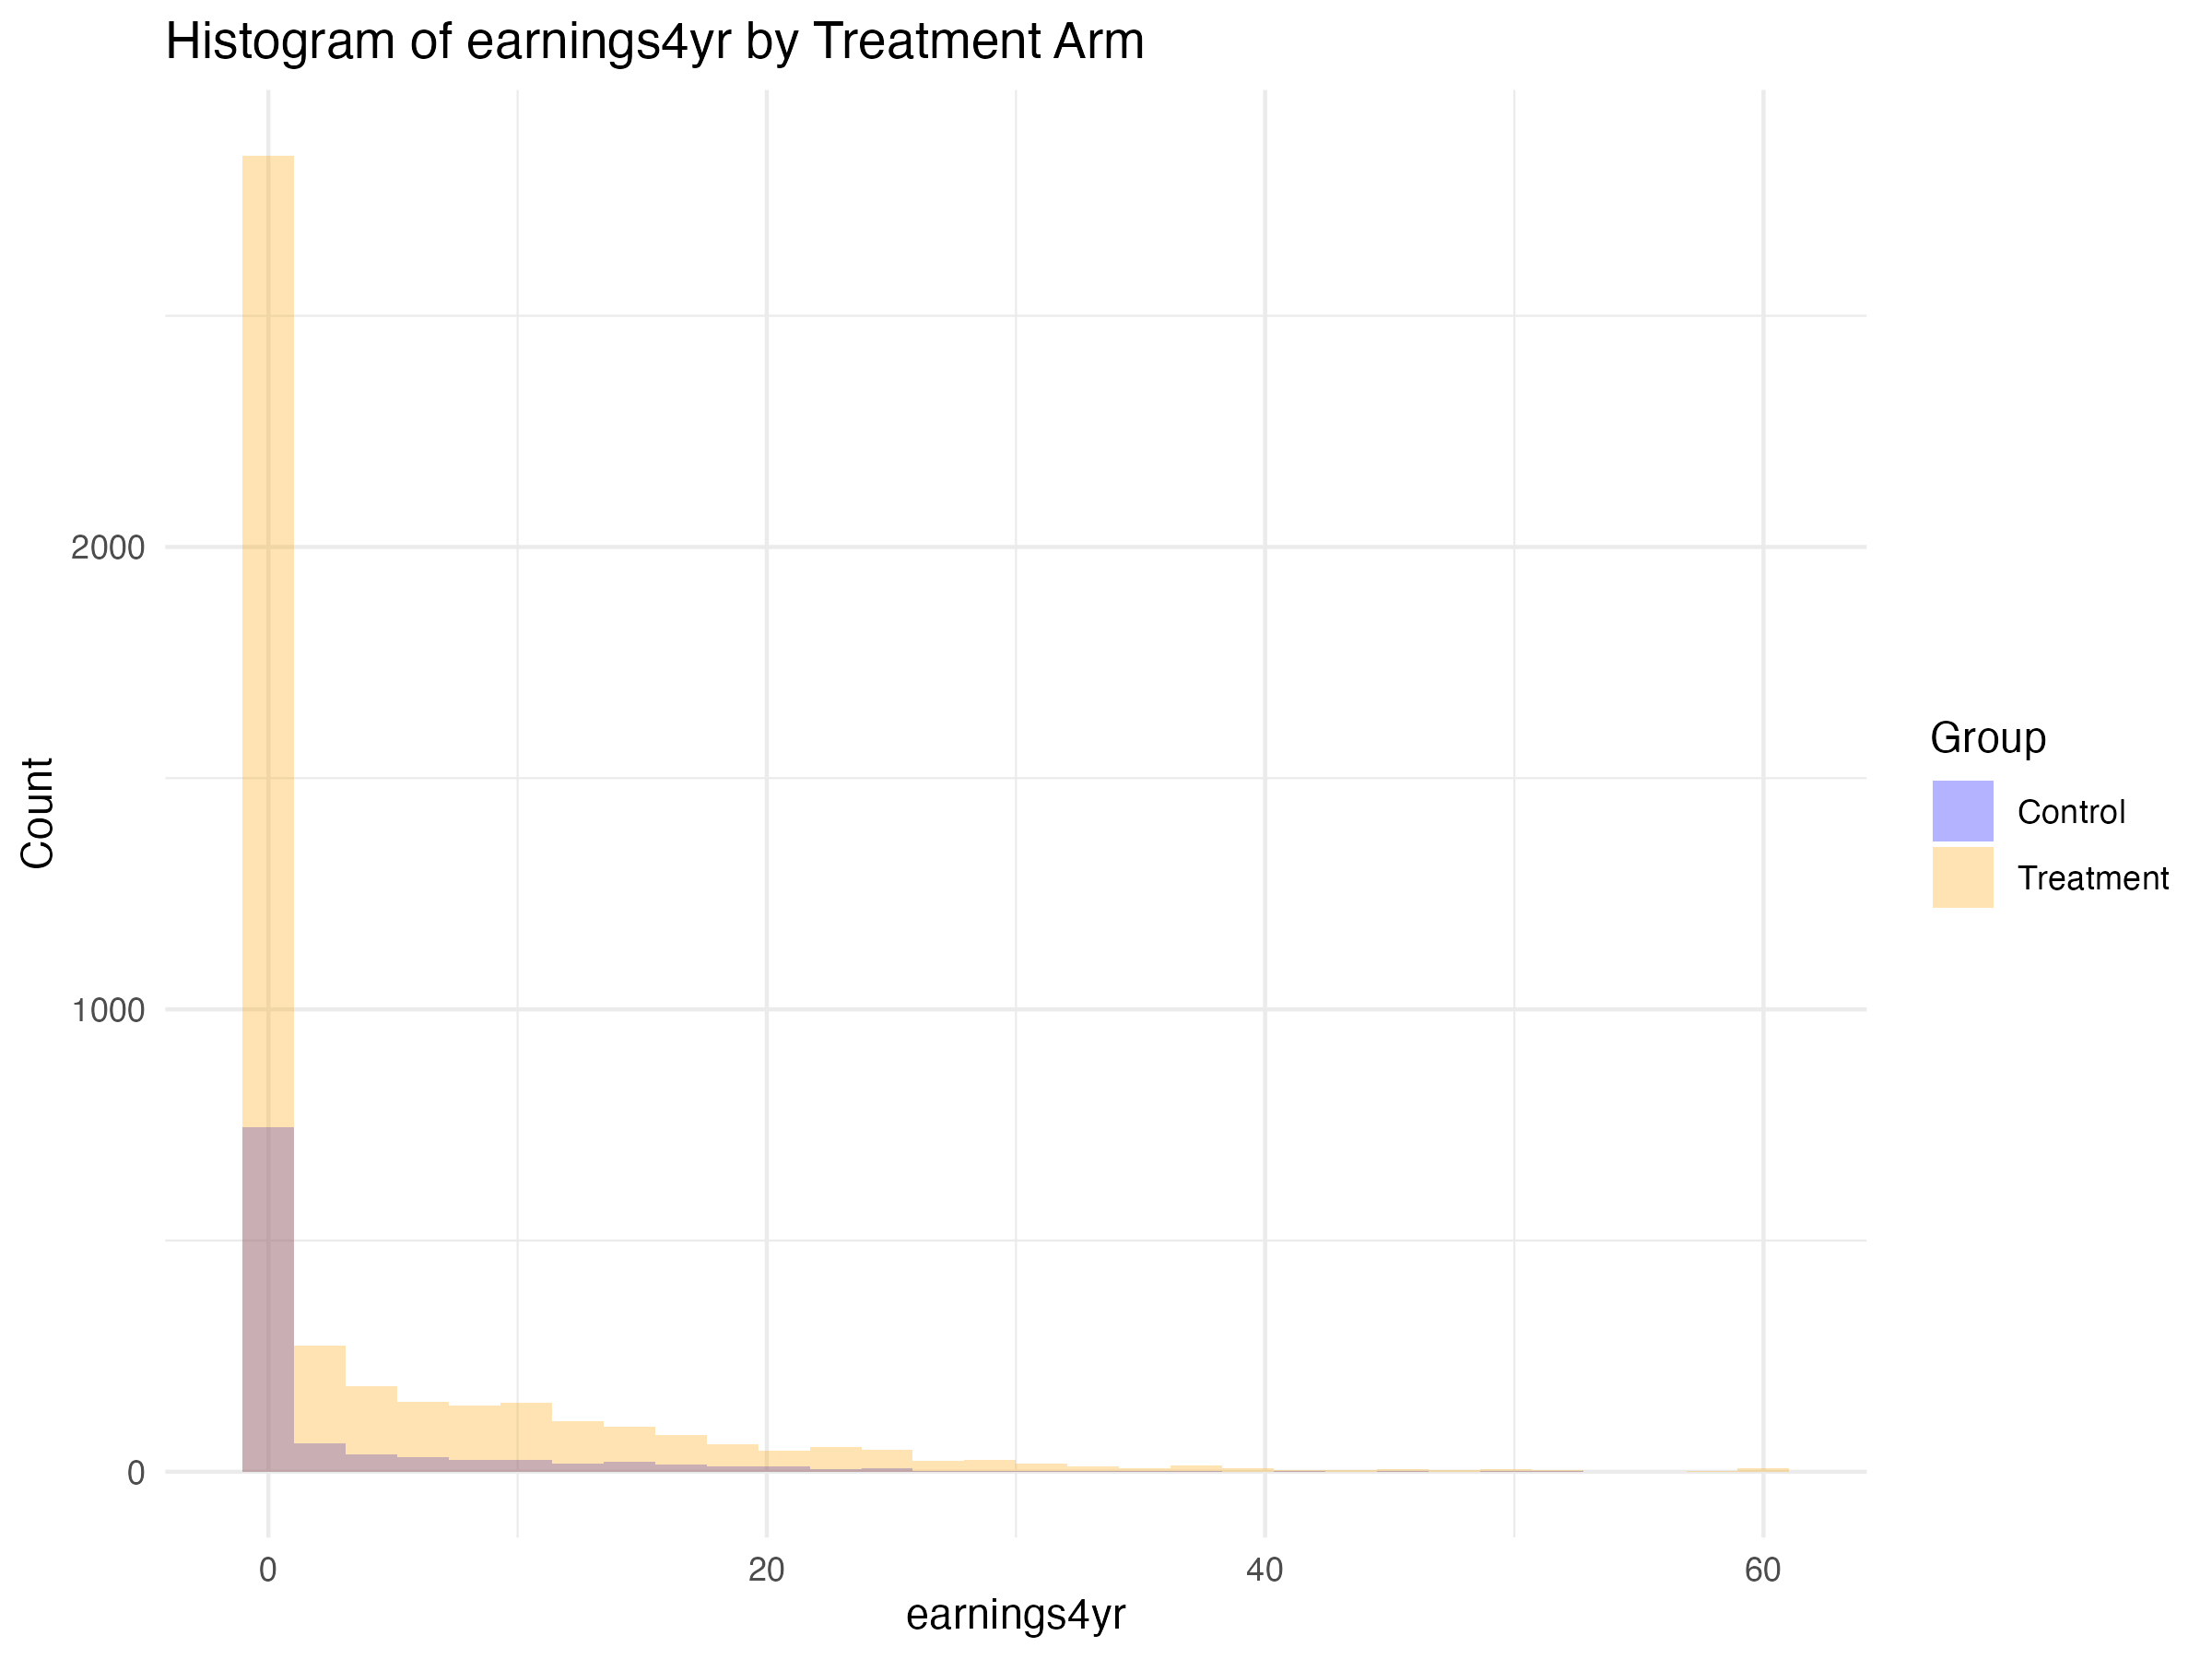
\includegraphics[width=0.8\textwidth]{output/histogram_earnings4yr_by_treatment_arm.png}
        \caption{\label{fig:hist_earnings4yr}Earnings four years after treatment}
    \end{subfigure}
    \caption{\label{fig:hist_earnings}Histograms of earnings one year and four years after treatment}
\end{figure}

\newpage

\subsection{(a) Plain Vanilla Bootstrap}

The plain vanilla bootstrap was implemented using the following approach in algorithm \ref{alg:bootstrap_sampling_process}.


\begin{algorithm}
    \caption{Bootstrap Sampling Process}
    \label{alg:bootstrap_sampling_process}
    For each bootstrap iteration $i \in \{1, 2, \ldots, B\}$ where $B = 100000$:
    \begin{enumerate}
    \item \textbf{Resampling}: Draw a bootstrap sample $d^{(i)}$ of size $n$ (original sample size) \textit{with replacement} from the original dataset. 
    
    \item \textbf{Compute Bootstrap Statistics}: For each bootstrap sample, calculate the difference-in-means (DIM) estimator:
    \begin{align}
        \hat{\tau}^{(i)}_1 &= \frac{1}{n^{(i)}_1} \sum_{j: W_j = 1} Y_{1j}^{(i)} - \frac{1}{n^{(i)}_0} \sum_{j: W_j = 0} Y_{1j}^{(i)} \\
        \hat{\tau}^{(i)}_4 &= \frac{1}{n^{(i)}_1} \sum_{j: W_j = 1} Y_{4j}^{(i)} - \frac{1}{n^{(i)}_0} \sum_{j: W_j = 0} Y_{4j}^{(i)}
    \end{align}
    where $Y_{1j}^{(i)}$ and $Y_{4j}^{(i)}$ are the earnings outcomes(1yr and 4yr) in the $i$-th bootstrap sample, and $n^{(i)}_1$, $n^{(i)}_0$ are the number of treated and control units in the bootstrap sample.
    
    \item \textbf{Store Bootstrap Estimates}: Collect all bootstrap estimates in vectors $\{\hat{\tau}^{(i)}_1\}_{i=1}^B$ and $\{\hat{\tau}^{(i)}_4\}_{i=1}^B$.
\end{enumerate}

Compute the bootstrap variance and the 90\% confidence intervals as follows:
\begin{align}
    \hat{V}_{boot,1} &= \frac{1}{B} \sum_{i=1}^B \left(\hat{\tau}^{(i)}_1 - \hat{\tau}_1\right)^2 \\
    \hat{V}_{boot,4} &= \frac{1}{B} \sum_{i=1}^B \left(\hat{\tau}^{(i)}_4 - \hat{\tau}_4\right)^2
\end{align}
where $\hat{\tau}_1$ and $\hat{\tau}_4$ are the original sample estimates.

The 90\% confidence intervals are constructed assuming normality:
\begin{align}
    \text{CI}_{90,1} &= \left[\hat{\tau}_1 - 1.645 \times \sqrt{\hat{V}_{boot,1}}, \hat{\tau}_1 + 1.645 \times \sqrt{\hat{V}_{boot,1}}\right] \\
    \text{CI}_{90,4} &= \left[\hat{\tau}_4 - 1.645 \times \sqrt{\hat{V}_{boot,4}}, \hat{\tau}_4 + 1.645 \times \sqrt{\hat{V}_{boot,4}}\right]
\end{align}
\end{algorithm}

\subsubsection{Results}


\begin{table}[h]
    \centering
    \begin{tabular}{lcc}
        \hline
         & earnings 1yr & earnings 4yr \\
        \hline
        DIM estimate & 1.1362  & 1.2323 \\
        Vanilla Bootstrap variance & 0.0179 & 0.0665 \\
        Confidence Intervals(90\%) & (0.9164, 1.3561) & (0.8081, 1.6565) \\
        \hline
    \end{tabular}
    \caption{\label{tab:bootstrap_results}Plain Vanilla Bootstrap Results}
\end{table}

The results are shown in table \ref{tab:bootstrap_results}.
The caveat for the plain vanilla bootstrap is that we might end up with a bootstrap sample that has either zero control units or zero treated units.
In this case, we might not be able to estimate the ATE without any modification to the bootstrap sampling process.


\subsection{(b) Bayesian Bootstrap}

The Bayesian bootstrap was implemented using the following approach in algorithm \ref{alg:bayesian_bootstrap_sampling_process}.


\begin{algorithm}
    \caption{Bayesian Bootstrap Sampling Process}
    \label{alg:bayesian_bootstrap_sampling_process}
    For each bootstrap iteration $i \in \{1, 2, \ldots, B\}$ where $B = 100000$:
    \begin{enumerate}
        \item \textbf{Generate Exponential Weights}: 
        \begin{align}
            E^{(i)}_j &\overset{iid}{\sim} \text{Exp}(1) \quad \text{for } j = 1, 2, \ldots, n
        \end{align}
        
        \item \textbf{Normalization of the weights}:
        \begin{align}
            R^{(i)}_j &= \frac{E^{(i)}_j}{\sum_{k=1}^n E^{(i)}_k}
        \end{align}
        

        \item \textbf{Compute Weighted Difference-in-Means}: Calculate the weighted difference-in-means estimator using the probability weights:
        \begin{align}
            \hat{\tau}^{(i)}_1 &= \frac{\sum_{j=1}^n R^{(i)}_j W_j Y_{1j}}{\sum_{j=1}^n R^{(i)}_j W_j} - \frac{\sum_{j=1}^n R^{(i)}_j (1-W_j) Y_{1j}}{\sum_{j=1}^n R^{(i)}_j (1-W_j)} \\
            \hat{\tau}^{(i)}_4 &= \frac{\sum_{j=1}^n R^{(i)}_j W_j Y_{4j}}{\sum_{j=1}^n R^{(i)}_j W_j} - \frac{\sum_{j=1}^n R^{(i)}_j (1-W_j) Y_{4j}}{\sum_{j=1}^n R^{(i)}_j (1-W_j)}
        \end{align}
        where $Y_{1j}$ and $Y_{4j}$ are the original earnings outcomes, and $W_j$ is the treatment indicator.
        
        \item \textbf{Store Bootstrap Estimates}: Collect all bootstrap estimates in vectors $\{\hat{\tau}^{(i)}_1\}_{i=1}^B$ and $\{\hat{\tau}^{(i)}_4\}_{i=1}^B$.
    \end{enumerate}
    
    Compute the Bayesian bootstrap variance and the 90\% confidence intervals as follows:
    \begin{align}
        \hat{V}_{bboot,1} &= \frac{1}{B} \sum_{i=1}^B \left(\hat{\tau}^{(i)}_1 - \hat{\tau}_1\right)^2 \\
        \hat{V}_{bboot,4} &= \frac{1}{B} \sum_{i=1}^B \left(\hat{\tau}^{(i)}_4 - \hat{\tau}_4\right)^2
    \end{align}
    where $\hat{\tau}_1$ and $\hat{\tau}_4$ are the original sample estimates.
    
    The 90\% confidence intervals are constructed assuming normality:
    \begin{align}
        \text{CI}_{90,1} &= \left[\hat{\tau}_1 - 1.645 \times \sqrt{\hat{V}_{bboot,1}}, \hat{\tau}_1 + 1.645 \times \sqrt{\hat{V}_{bboot,1}}\right] \\
        \text{CI}_{90,4} &= \left[\hat{\tau}_4 - 1.645 \times \sqrt{\hat{V}_{bboot,4}}, \hat{\tau}_4 + 1.645 \times \sqrt{\hat{V}_{bboot,4}}\right]
    \end{align}
\end{algorithm}

\subsubsection{Results}

The results are shown in table \ref{tab:bayesian_bootstrap_results}.
The caveat for the Bayesian bootstrap is that we might end up with a bootstrap sample that has either zero control units or zero treated units.
In this case, we might not be able to estimate the ATE without any modification to the bootstrap sampling process.

\begin{table}[h]
    \centering
    \begin{tabular}{lcc}
        \hline
         & earnings 1yr & earnings 4yr \\
        \hline
        DIM estimate & 1.1362  & 1.2323 \\
        Bayesian Bootstrap variance &  0.0168 & 0.0599 \\
        Confidence Intervals(90\%) & (0.9232, 1.3492) & (0.8296, 1.6350) \\
        \hline
    \end{tabular}
    \caption{\label{tab:bayesian_bootstrap_results}Bayesian Bootstrap Results}
\end{table}


\subsection{(c) Percentile Bootstrap with t-stats}



Here, I follow the exact same procedures in algorithms \ref{alg:bootstrap_sampling_process} and \ref{alg:bayesian_bootstrap_sampling_process} but construct the confidence intervals with the 0.05 and 0.95 quantiles of the bootstrap t-statistic from step 3 instead of plugging in the bootstrap standard error to the normal distribution.

\subsubsection{Results}

The results are shown in table \ref{tab:percentile_bootstrap_results}.


\begin{table}[h]
    \centering
    \begin{tabular}{lcc}
        \hline
         & earnings 1yr & earnings 4yr \\
        \hline
        DIM estimate & 1.1362  & 1.2323 \\
        Percentile Bootstrap Confidence Intervals(90\%) & (0.9044, 1.3370) & (0.7862, 1.6615) \\
        Percentile Bayesian Bootstrap Confidence Intervals(90\%) & (0.9208, 1.3484) & (0.8448, 1.6419) \\
        \hline
    \end{tabular}
    \caption{\label{tab:percentile_bootstrap_results}Percentile Bootstrap Results with t-stats}
\end{table}

The 0.05 and 0.95 percentiles for the bootstrap t-stats are 0.9044 and 1.3370, respectively.

\subsection{(d) Subsampling}

The subsampling bootstrap was implemented using the following approach:

\subsubsection{Subsampling Bootstrap Process}

\begin{algorithm}
    \caption{Subsampling Bootstrap Process}
    \label{alg:subsampling_bootstrap_process}
    \begin{enumerate}
        \item \textbf{Determine Subsample Size}: Set the subsample size to be the square root of the original sample size$(n)$:
        \begin{align}
            m &= \text{round}(\sqrt{n})
        \end{align}
        
        \item \textbf{Subsampling}: For each bootstrap iteration $i \in \{1, 2, \ldots, B\}$ where $B = 1000$:
        \begin{itemize}
            \item Draw a subsample of size $m$ \textit{without replacement} from the original dataset
            \item Compute the difference-in-means (DIM) estimator on this subsample:
            \begin{align}
                \hat{\tau}^{(i)}_1 &= \frac{1}{m^{(i)}_1} \sum_{j: W_j = 1} Y_{1j}^{(i)} - \frac{1}{m^{(i)}_0} \sum_{j: W_j = 0} Y_{1j}^{(i)} \\
                \hat{\tau}^{(i)}_4 &= \frac{1}{m^{(i)}_1} \sum_{j: W_j = 1} Y_{4j}^{(i)} - \frac{1}{m^{(i)}_0} \sum_{j: W_j = 0} Y_{4j}^{(i)}
            \end{align}
            where $m^{(i)}_1$ and $m^{(i)}_0$ are the number of treated and control units in the $i$-th subsample.
        \end{itemize}
        
        \item \textbf{Scale the Variance}: The subsampling variance is scaled by the ratio of subsample size to original sample size:
        \begin{align}
            \hat{V}_{sub,1} &= \frac{m}{n} \cdot \frac{1}{B} \sum_{i=1}^B \left(\hat{\tau}^{(i)}_1 - \hat{\tau}_1\right)^2 \\
            \hat{V}_{sub,4} &= \frac{m}{n} \cdot \frac{1}{B} \sum_{i=1}^B \left(\hat{\tau}^{(i)}_4 - \hat{\tau}_4\right)^2
        \end{align}
        where $\hat{\tau}_1$ and $\hat{\tau}_4$ are the original sample estimates.
        
        \item \textbf{Construct Confidence Intervals}: The 90\% confidence intervals are:
        \begin{align}
            \text{CI}_{90,1} &= \left[\hat{\tau}_1 - 1.645 \times \sqrt{\hat{V}_{sub,1}}, \hat{\tau}_1 + 1.645 \times \sqrt{\hat{V}_{sub,1}}\right] \\
            \text{CI}_{90,4} &= \left[\hat{\tau}_4 - 1.645 \times \sqrt{\hat{V}_{sub,4}}, \hat{\tau}_4 + 1.645 \times \sqrt{\hat{V}_{sub,4}}\right]
        \end{align}
    \end{enumerate}
\end{algorithm}

\subsubsection{Results}

The results are shown in table \ref{tab:subsampling_bootstrap_results}.

\begin{table}[h]
    \centering
    \begin{tabular}{lcc}
        \hline
         & earnings 1yr & earnings 4yr \\
        \hline
        Subsampling Bootstrap Varaince & 0.0186 & 0.0646 \\
        Subsampling Bootstrap Confidence Intervals(90\%) & (0.9121, 1.3602) & (0.8142, 1.6505) \\
        \hline
    \end{tabular}
    \caption{\label{tab:subsampling_bootstrap_results}Subsampling Bootstrap Results}
\end{table}

\subsection{(e) OLS Regression}

To estimate the average treatment effect while adjusting for whether individuals have a high school degree, I use an interacted linear regression (OLS) approach. 
This estimator allows for heterogeneous treatment effects across different education groups.

\begin{align}
    Y_i = \beta_0 + \beta_1 W_i + \beta_2 \text{hs\_diploma}_i + \beta_3 W_i \times \text{hs\_diploma}_i + \epsilon_i
\end{align}

\begin{itemize}
    \item $Y_i$ is the earnings outcome (1-year or 4-year)
    \item $W_i$ is the treatment indicator
    \item $\text{hs\_diploma}_i$ is the high school diploma indicator
    \item The average treatment effect is $\beta_1 + \beta_3 \cdot \mathbb{E}[\text{hs\_diploma}]$
\end{itemize}

\subsubsection{Motivation for the Estimator}

I choose the interacted OLS regression for the following reasons:

\begin{itemize}
    \item \textbf{Heterogeneous Treatment Effects}: The model allows the treatment effect to vary by high school diploma status, capturing potential differences in program effectiveness across education groups.
    
    \item \textbf{Regression Adjustment}: By including the interaction term $W \times \text{hs\_diploma}$, we can control for baseline differences between education groups while estimating the average treatment effect.
    
    \item \textbf{Prediction by Group}: If the model is well-specified, we can predict the earnings outcome by the high school diploma status and the treatment indicator. Even if the true relationship is non-linear, OLS provides a good linear approximation that is robust and interpretable.
\end{itemize}


\subsubsection{Parametric Bootstrap Process}

\begin{algorithm}
    \caption{Parametric Bootstrap for OLS Regression}
    \label{alg:parametric_bootstrap_ols}
    \begin{enumerate}
        \item \textbf{Estimate Original Model}: Fit the OLS regression on the original data:
        \begin{align}
            \hat{Y}_i = \hat{\beta}_0 + \hat{\beta}_1 W_i + \hat{\beta}_2 \text{hs\_diploma}_i + \hat{\beta}_3 W_i \times \text{hs\_diploma}_i
        \end{align}
        
        \item \textbf{Calculate Original ATE}: Compute the average treatment effect:
        \begin{align}
            \widehat{ATE} = \hat{\beta}_1 + \hat{\beta}_3 \cdot \bar{p}_{hs}
        \end{align}
        where $\bar{p}_{hs} = \frac{1}{n}\sum_{i=1}^n \text{hs\_diploma}_i$ is the sample proportion with high school diploma.
        
        \item \textbf{Extract Components}: Store the estimated coefficients $\hat{\beta}$, residuals $\hat{\epsilon}_i = Y_i - \hat{Y}_i$, and covariates $(W_i, \text{hs\_diploma}_i)$.
        
        \item \textbf{Bootstrap Resampling}: For each bootstrap iteration $i \in \{1, 2, \ldots, B\}$ where $B = 1000$:
        \begin{itemize}
            \item Resample residuals with replacement: $\epsilon^{(i)}_j \sim \{\hat{\epsilon}_1, \ldots, \hat{\epsilon}_n\}$
            \item Generate bootstrap outcomes using the estimated model:
            \begin{align}
                Y^{(i)}_j = \hat{\beta}_0 + \hat{\beta}_1 W_j + \hat{\beta}_2 \text{hs\_diploma}_j + \hat{\beta}_3 W_j \times \text{hs\_diploma}_j + \epsilon^{(i)}_j
            \end{align}
            \item Refit the OLS regression on the bootstrap data: $Y^{(i)}_j \sim W_j + \text{hs\_diploma}_j + W_j \times \text{hs\_diploma}_j$
            \item Calculate the bootstrap ATE:
            \begin{align}
                \widehat{ATE}^{(i)} = \hat{\beta}^{(i)}_1 + \hat{\beta}^{(i)}_3 \cdot \bar{p}_{hs}
            \end{align}
            where $\hat{\beta}^{(i)}_1$ and $\hat{\beta}^{(i)}_3$ are the bootstrap coefficient estimates.
        \end{itemize}
        
        \item \textbf{Estimate ATE Variance}: Compute the parametric bootstrap variance of the ATE:
        \begin{align}
            \hat{V}_{boot, ATE} = \frac{1}{B} \sum_{i=1}^B \left(\widehat{ATE}^{(i)} - \widehat{ATE}\right)^2
        \end{align}
        
        \item \textbf{Construct Confidence Intervals}: For 95\% confidence intervals:
        \begin{align}
            \text{CI}_{95, ATE} = \left[\widehat{ATE} - 1.96 \times \sqrt{\hat{V}_{boot, ATE}}, \widehat{ATE} + 1.96 \times \sqrt{\hat{V}_{boot, ATE}}\right]
        \end{align}
    \end{enumerate}
\end{algorithm}

% \subsubsection{Advantages of Parametric Bootstrap}

% \begin{itemize}
%     \item \textbf{Model-Based}: Assumes the linear model is correctly specified, which can provide more precise estimates when the model is appropriate.
    
%     \item \textbf{Residual Resampling}: By resampling residuals rather than observations, it preserves the structure of covariates while accounting for uncertainty in the error term.
    
%     \item \textbf{Computational Efficiency}: More efficient than non-parametric bootstrap as it doesn't require refitting models with varying sample compositions.
    
%     \item \textbf{Theoretical Foundation}: Well-grounded in classical regression theory and provides valid inference under standard regression assumptions.
% \end{itemize}

\newpage

\subsubsection{Results}

The results are shown in table \ref{tab:ols_regression_results}.
As a side note, it must be noted that the ratio of individuals with high school diploma in our sample 
is treated as the population proportion with high school diploma for the bootstrap procedure. This follows the same logic that the bootstrap procedure inherently has.
Also, just for the sake of comparison with other bootstrap procedures, I report the 90\% confidence intervals as well.

\begin{table}[h]
    \centering
    \begin{tabular}{lcc}
        \hline
         & earnings 1yr & earnings 4yr \\
        \hline
        Average Treatment Effect & 1.136 & 1.232 \\
        Proportion with HS Diploma & 0.523 & 0.523 \\
        Parametric Bootstrap SE (ATE) & 0.169 & 0.277 \\
        90\% CI for ATE & [0.858, 1.414] & [0.776, 1.689] \\
        95\% CI for ATE & [0.805, 1.468] & [0.689, 1.776] \\
        \hline
    \end{tabular}
    \caption{\label{tab:ols_regression_results}OLS Regression with Parametric Bootstrap Results}
\end{table}


\subsubsection{Comparison of Different Bootstrap Procedures}


Figure~\ref{fig:bootstrap_comparison} presents a comparison of several bootstrap methods for estimating 90\% confidence intervals for the treatment effect, both for 1-year and 4-year log-earnings outcomes. The methods compared include the vanilla (nonparametric) bootstrap, Bayesian bootstrap, percentile bootstrap, subsampling bootstrap, and the OLS parametric bootstrap.

\begin{figure}[h]
    \centering
    \begin{subfigure}{0.48\textwidth}
    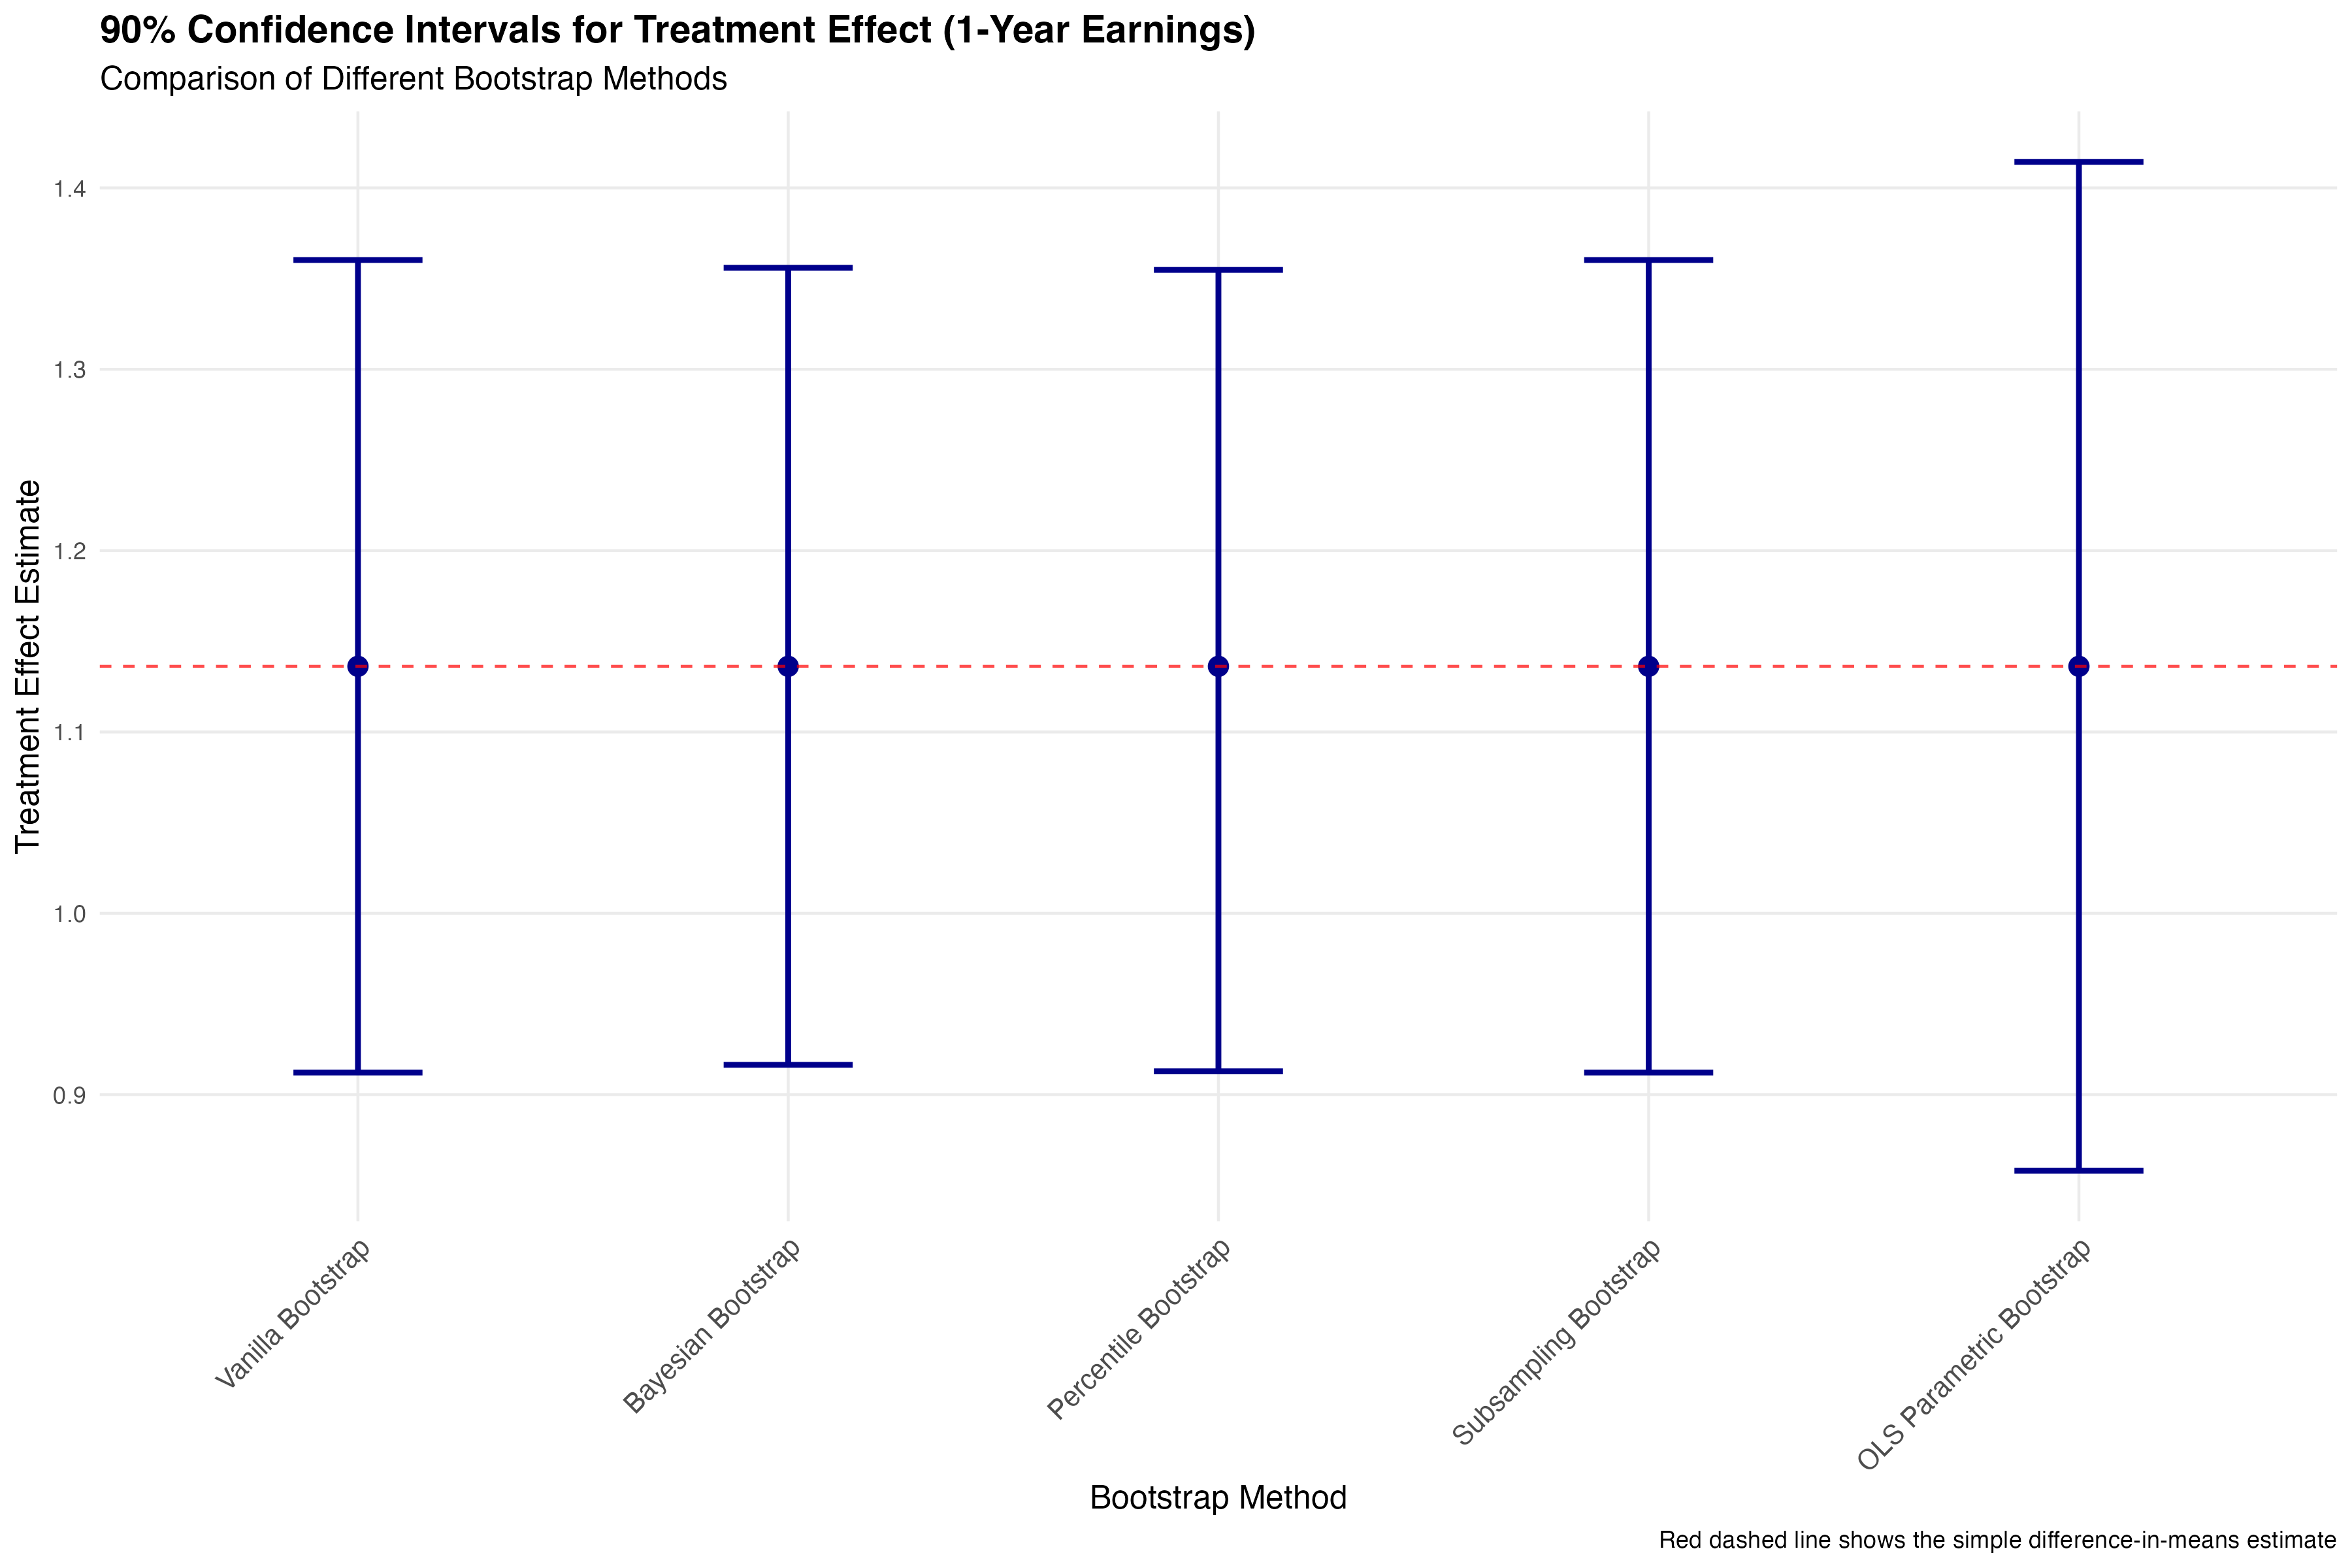
\includegraphics[width=\textwidth]{output/bootstrap_comparison_1yr.png}
    \caption{\label{fig:bootstrap_comparison_1yr}for 1-year earnings}
    \end{subfigure}
    \begin{subfigure}{0.48\textwidth}
    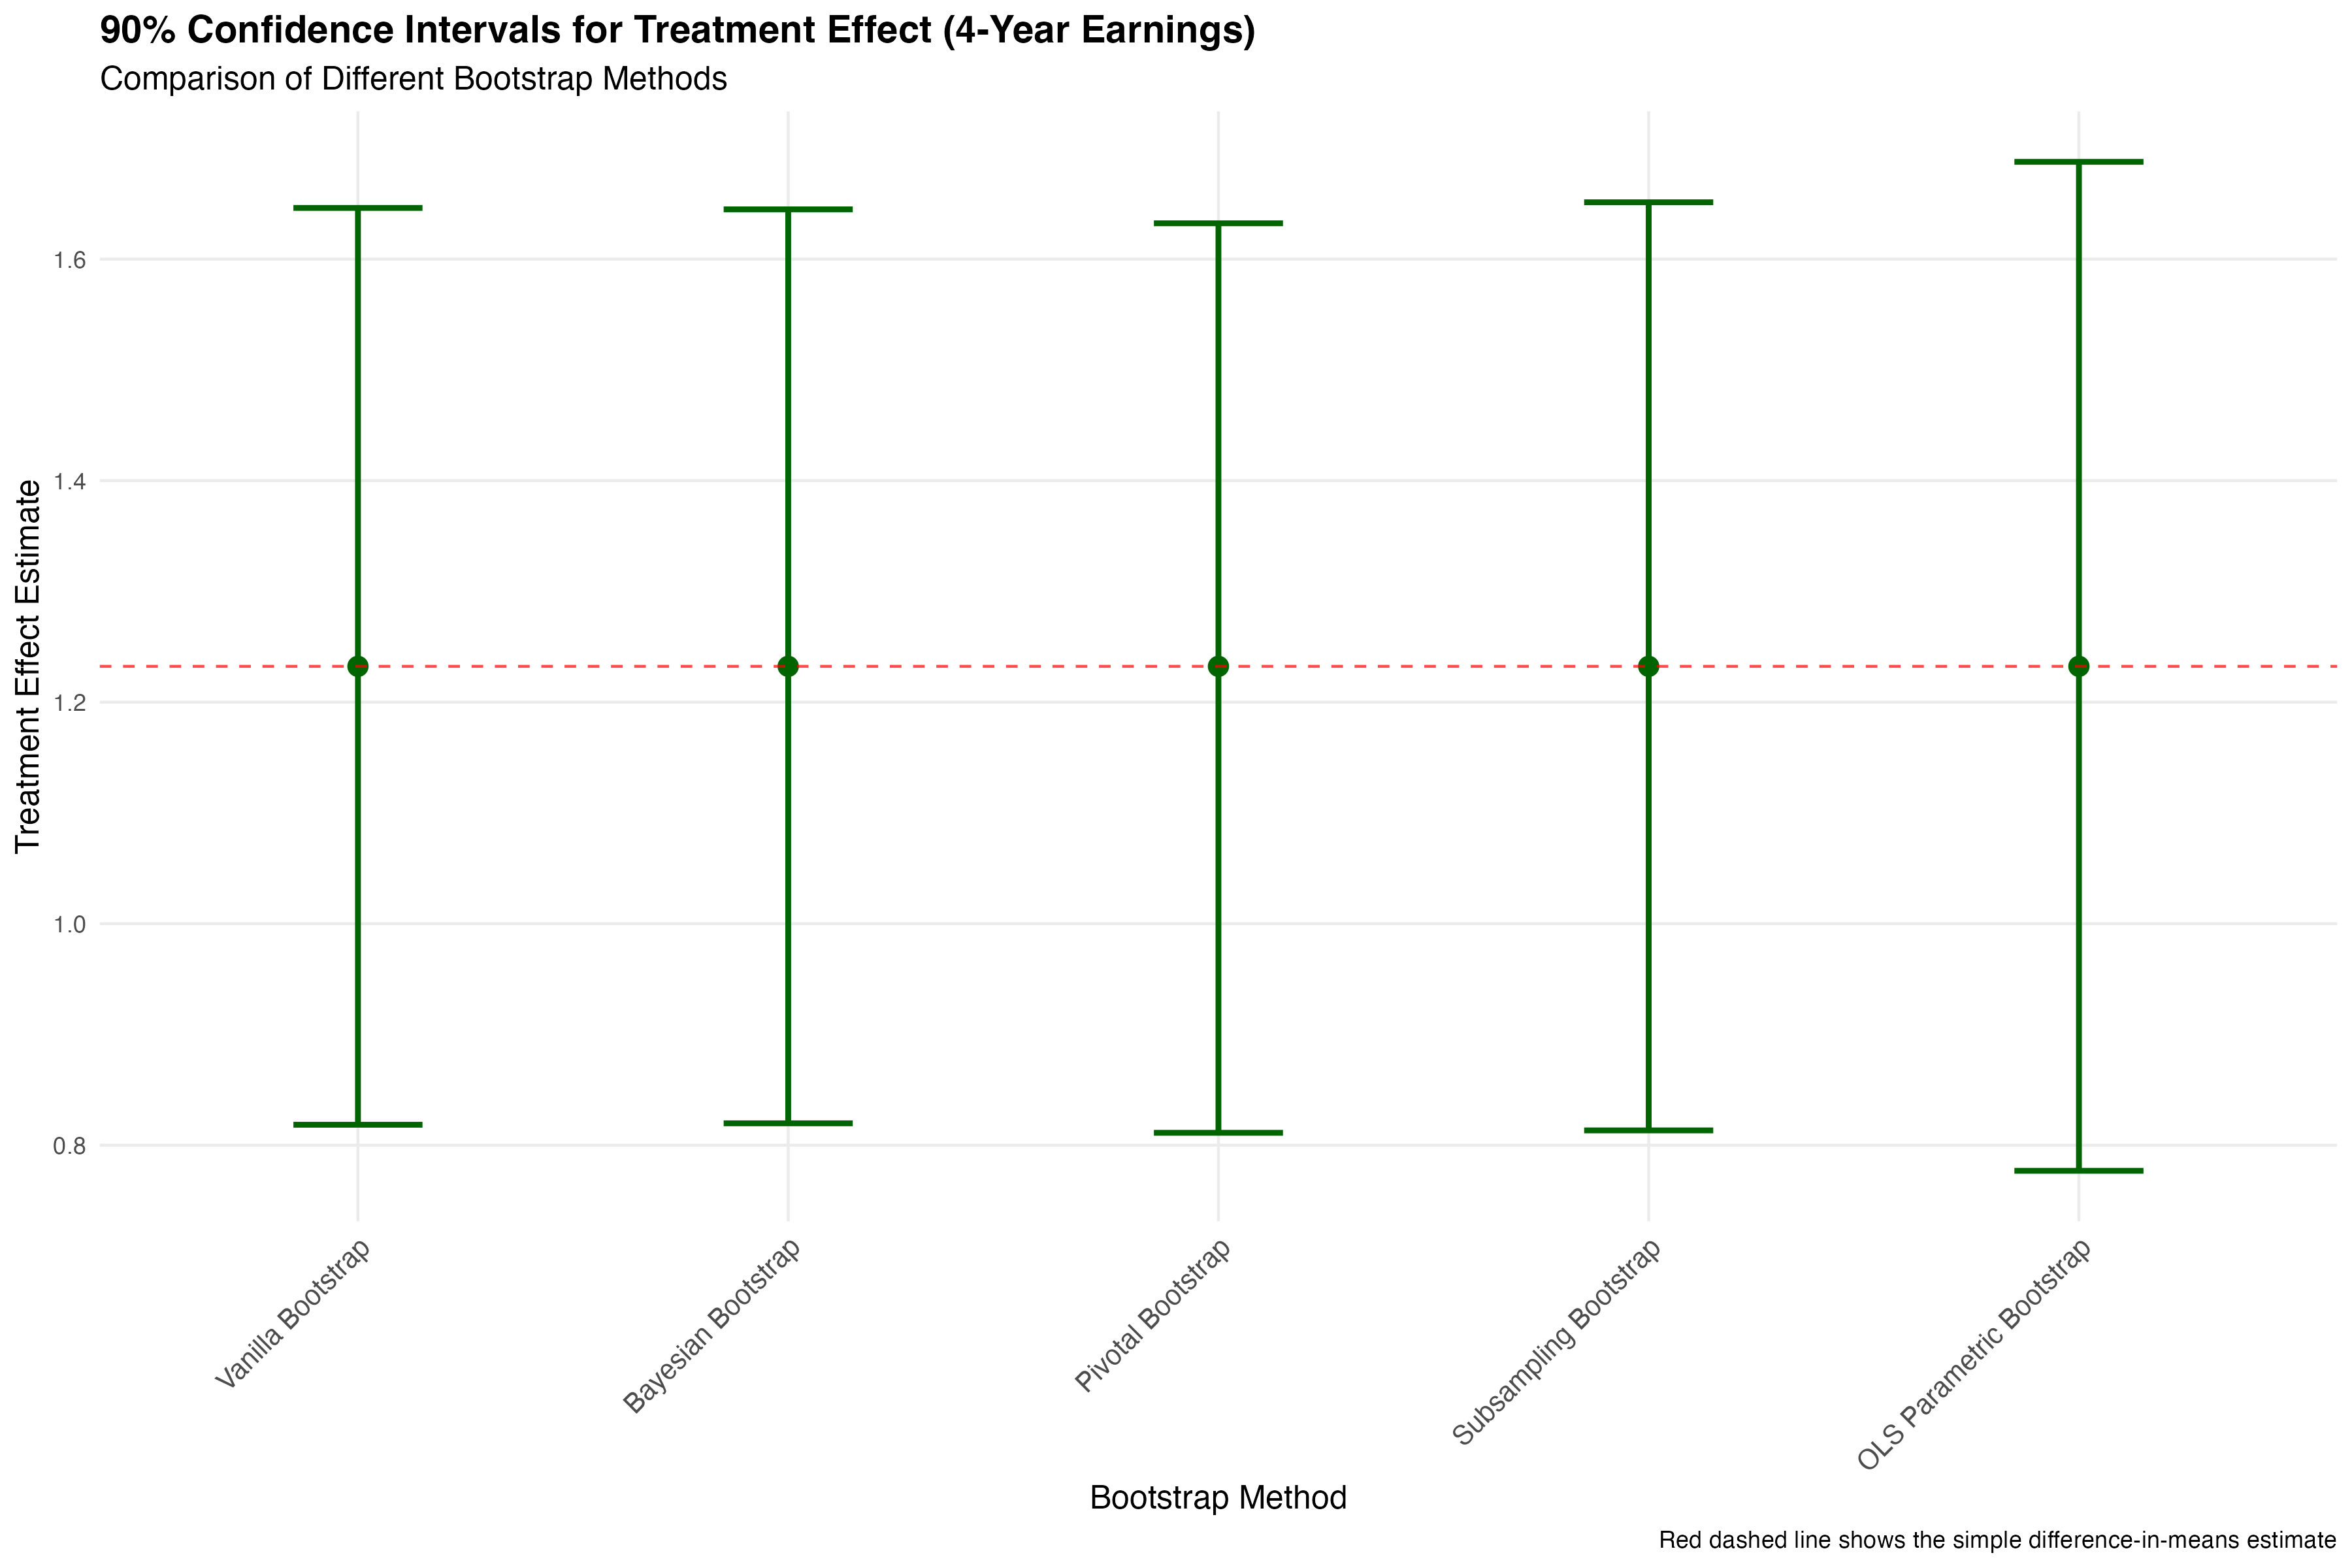
\includegraphics[width=\textwidth]{output/bootstrap_comparison_4yr.png}
    \caption{\label{fig:bootstrap_comparison_4yr}for 4-year earnings}
    \end{subfigure}
    \caption{\label{fig:bootstrap_comparison}Comparison of Different Bootstrap Procedures}
\end{figure}






\section{Part II}



\subsection{(a) Estimator Choice}


I would choose the \textbf{average of the difference between treated and controls in the old group and the difference between treated and controls in the young group}.\footnote{Note that if the size of the young and old groups are different, we can use the weighted average instead of the average, where the weights are determined by the proportions of old and young individuals in the sample.}


Suppose we have a random sample $(W_i, A_i, Y_i(1), Y_i(0))$ from the population, where $W_i$ is the treatment indicator, $A_i$ is the age group indicator(1 if old), $Y_i(1)$ and $Y_i(0)$ are the potential outcomes, and $Y_i = W_iY_i(1) + (1-W_i)Y_i(0)$ is the observed outcome.
Let $n_{old} = 50$ and $n_{young} = 50$ be the population sizes, and $n_{old,treat} = 27$, $n_{young,treat} = 23$, $n_{old,control} = 23$, $n_{young,control} = 27$ be the group sizes after treatment assignment.

The two estimators are:

\begin{align}
\hat{\tau}_{DIM} &= \frac{1}{50} \sum_{i \in \text{Treatment}} Y_i - \frac{1}{50} \sum_{i \in \text{Control}} Y_i \\
&= \sum_{i=1}^{50}\frac{W_iY_i(1)}{\sum_{i=1}^{50}W_i} - \sum_{i=1}^{50}\frac{(1-W_i)Y_i(0)}{\sum_{i=1}^{50}(1-W_i)}\notag\\
\hat{\tau}_{avg} &= \frac{50}{100} \left(\frac{1}{27} \sum_{i \in \text{Treatment, Old}} Y_i - \frac{1}{23} \sum_{i \in \text{Control, Old}} Y_i\right) \\
&\quad + \frac{50}{100} \left(\frac{1}{23} \sum_{i \in \text{Treatment, Young}} Y_i - \frac{1}{27} \sum_{i \in \text{Control, Young}} Y_i\right)\notag\\
&= \frac{50}{100}\biggl(\sum_{i=1}^{50}\frac{W_iA_iY_i(1)}{\sum_{i=1}^{50}W_iA_i} - \sum_{i=1}^{50}\frac{(1-W_i)A_iY_i(0)}{\sum_{i=1}^{50}(1-W_i)A_i}\biggr)\notag\\
&\quad + \frac{50}{100}\biggl(\sum_{i=1}^{50}\frac{W_i(1-A_i)Y_i(1)}{\sum_{i=1}^{50}W_i(1-A_i)} - \sum_{i=1}^{50}\frac{(1-W_i)(1-A_i)Y_i(0)}{\sum_{i=1}^{50}(1-W_i)(1-A_i)}\biggr)\notag
\end{align}

\subsubsection{Variance of \texorpdfstring{$\hat{\tau}_{avg}$}{tau\_avg}}

Since the strata represent independent samples, the variance of $\hat{\tau}_{avg}$ is:
\begin{align}
\Var(\hat{\tau}_{avg}) = (0.5)^2 \Var(\hat{\tau}_{old}) + (0.5)^2 \Var(\hat{\tau}_{young})
\end{align}

assuming (or condition on) the ratio of young and old to be fixed.

The variance of the estimator within the old stratum is:
\begin{align}
\Var(\hat{\tau}_{old}) = \Var(\bar{Y}_{treat,old}) + \Var(\bar{Y}_{control,old}) = \frac{\Var(Y_i(1)|A_i=1)}{n_{old,treat}} + \frac{\Var(Y_i(0)|A_i=1)}{n_{old,control}} = \frac{\sigma^2_1(1)}{25} + \frac{\sigma^2_0(1)}{25}
\end{align}
where $\sigma^2_w(a) = \Var(Y_i(w)|A_i=a)$. Similarly, $\Var(\hat{\tau}_{young}) = \frac{\sigma^2_1(0)}{25} + \frac{\sigma^2_0(0)}{25}$.
Substituting these into the main variance formula yields:
\begin{align}
\Var(\hat{\tau}_{avg}) &= \frac{1}{4} \left( \frac{\sigma^2_1(1) + \sigma^2_0(1)}{25} + \frac{\sigma^2_1(0) + \sigma^2_0(0)}{25} \right) \\
&= \frac{1}{100} \left( \sigma^2_1(1) + \sigma^2_0(1) + \sigma^2_1(0) + \sigma^2_0(0) \right)
\end{align}

\subsubsection{Variance of \texorpdfstring{$\hat{\tau}_{DIM}$}{tau\_DIM}}

Under the balanced design, $W_i$ is independent of potential outcomes, so $\Var(Y_i|W_i=1) = \Var(Y_i(1))$ and $\Var(Y_i|W_i=0) = \Var(Y_i(0))$. With total sample sizes $n_{treat}=n_{control}=50$:
\begin{align}
\Var(\hat{\tau}_{DIM}) = \frac{\Var(Y_i(1))}{50} + \frac{\Var(Y_i(0))}{50}
\end{align}
Using the law of total variance, we can decompose the variance of each potential outcome:
\begin{align}
\Var(Y_i(1)) = \E[\Var(Y_i(1)|A_i)] + \Var(\E[Y_i(1)|A_i])
\end{align}
The two components of this decomposition are:
\begin{itemize}
    \item $\E[\Var(Y_i(1)|A_i)] = P(A_i=1)\sigma^2_1(1) + P(A_i=0)\sigma^2_1(0) = 0.5\sigma^2_1(1) + 0.5\sigma^2_1(0)$
    \item $\Var(\E[Y_i(1)|A_i]) = P(A=1)P(A=0)(\mu_{1,old} - \mu_{1,young})^2 = 0.25(\mu_{1,old} - \mu_{1,young})^2$, where we define $\mu_{w,a} = \E[Y_i(w)|A_i=a]$.
\end{itemize}
Combining these results for both $Y_i(1)$ and $Y_i(0)$:

\begin{align*}
\Var(\hat{\tau}_{DIM}) &= \frac{1}{50} \left[ \left(0.5(\sigma^2_1(1) + \sigma^2_1(0)) + 0.25(\mu_{1,old}-\mu_{1,young})^2\right) \right. \\
&\quad \left. + \left(0.5(\sigma^2_0(1) + \sigma^2_0(0)) + 0.25(\mu_{0,old}-\mu_{0,young})^2\right) \right] \\
&= \frac{1}{100} (\sigma^2_1(1) + \sigma^2_1(0) + \sigma^2_0(1) + \sigma^2_0(0)) \\
&\quad + \frac{1}{200} \left( (\mu_{1,old}-\mu_{1,young})^2 + (\mu_{0,old}-\mu_{0,young})^2 \right)
\end{align*}

\subsubsection{Comparison}

By inspecting the final variance expressions for the two estimators, we can see the direct relationship between them:
\begin{align}
\Var(\hat{\tau}_{DIM}) = \Var(\hat{\tau}_{avg}) + \frac{1}{200} \left[ (\mu_{1,old}-\mu_{1,young})^2 + (\mu_{0,old}-\mu_{0,young})^2 \right]
\end{align}
The second term on the right-hand side is a sum of squared differences, which is always non-negative. Therefore, we can conclude that:
\begin{align}
\Var(\hat{\tau}_{DIM}) \ge \Var(\hat{\tau}_{avg})
\end{align}

Therefore, I will choose the stratified estimator $\hat{\tau}_{avg}$ over the difference-in-means estimator $\hat{\tau}_{DIM}$ because it is \textit{more efficient}.

\subsection{(b) Unbiasedness}



\subsubsection{Difference-in-means}

\begin{align}
    \E[\hat{\tau}_{DIM}] &= \E\biggl[\frac{1}{50}\sum_{i=1}^{50}W_iY_i\biggr] - \E\biggl[\frac{1}{50}\sum_{i=1}^{50}(1-W_i)Y_i\biggr]\\
    &=\underbrace{ \E\biggl[\frac{1}{50}\sum_{i=1}^{50}W_iY_i(1)\biggr] - \E\biggl[\frac{1}{50}\sum_{i=1}^{50}(1-W_i)Y_i(0)\biggr]}_\text{by the independence of $W_i$ and $\{Y_i(1), Y_i(0)\}$}\\
    &= \E[Y_i(1) | W_i=1] - \E[Y_i(0) | W_i=0] = \E[Y_i(1)] - \E[Y_i(0)] = \tau
\end{align}

\subsubsection{Stratified Estimator}

First, we know that

\begin{align}
    \tau &= 0.5\tau_{old} + 0.5\tau_{young}\\
    \hat{\tau}_{avg} &= 0.5 \left(\bar{Y}_{treat,old} - \bar{Y}_{control,old}\right) + 0.5 \left(\bar{Y}_{treat,young} - \bar{Y}_{control,young}\right) 
\end{align}

since the experiment was carried out in a 50-50 split random assignment.

Because the treatment assignment is random, we have the following equalities:
\begin{align}
    \E[\bar{Y}_{treat,old}] &= \E[Y_i(1) | A_i=1] \\
    \E[\bar{Y}_{control,old}] &= \E[Y_i(0) | A_i=1]
\end{align}

Therefore,

\begin{align}
    \E[\bar{Y}_{treat,old} - \bar{Y}_{control,old}] &= \E[Y_i(1) | A_i=1] - \E[Y_i(0) | A_i=1] = \tau_{old}\\
    \E[\bar{Y}_{treat,young} - \bar{Y}_{control,young}] &= \E[Y_i(1) | A_i=0] - \E[Y_i(0) | A_i=0] = \tau_{young}
\end{align}

and thus $\E[\hat{\tau}_{avg}] = 0.5\tau_{old} + 0.5\tau_{young} = \tau$.



%---- Appendix -----------------
\appendix
\setcounter{figure}{0}                      
\setcounter{table}{0}                      
\renewcommand\thefigure{A.\arabic{figure}} 
\renewcommand\thetable{A.\arabic{table}} 

\begin{sidewaystable}[h]
    \centering
    \tiny
    
\begin{tabular}{lrrrrrrrrrrrrrrrr}
\toprule
variable & numNA & numZeros & fracZeros & mean & sd & min & max & 10\% & 20\% & 30\% & 40\% & 50\% & 90\% & 95\% & 99\% & 99.9\%\\
\midrule
educ & 0 & 598 & 0.0018 & 12.7699 & 3.2812 & 0.0000 & 20.0000 & 9.0000 & 11.0000 & 12.0000 & 12.0000 & 12.0000 & 17.0000 & 19.0000 & 20.000 & 20.0000\\
lwage & 0 & 3 & 0.0000 & 5.8999 & 0.6788 & -2.3418 & 10.5321 & 5.2343 & 5.5218 & 5.7243 & 5.8472 & 5.9525 & 6.5567 & 6.8004 & 7.274 & 7.9495\\
yob & 0 & 0 & 0.0000 & 34.6028 & 2.9050 & 30.0000 & 39.0000 & 30.0000 & 32.0000 & 33.0000 & 34.0000 & 35.0000 & 39.0000 & 39.0000 & 39.000 & 39.0000\\
\bottomrule
\end{tabular}

    \caption{\label{tab:summary_stats}Summary Statistics}
\end{sidewaystable}


\begin{sidewaystable}[h]
    \centering
    \tiny
    
\begin{tabular}{lrrrrrrrrrrrrrrrr}
\toprule
variable & numNA & numZeros & fracZeros & mean & sd & min & max & 10\% & 20\% & 30\% & 40\% & 50\% & 90\% & 95\% & 99\% & 99.9\%\\
\midrule
W & 0 & 1,036 & 1.0000 & 0.0000 & 0.0000 & 0.0000 & 0.0000 & 0.0000 & 0.0000 & 0.0000 & 0.0000 & 0.0000 & 0.0000 & 0.0000 & 0.0000 & 0.0000\\
earnings1yr & 0 & 679 & 0.6554 & 1.4493 & 3.4950 & 0.0000 & 34.5994 & 0.0000 & 0.0000 & 0.0000 & 0.0000 & 0.0000 & 5.1112 & 8.6316 & 16.3443 & 28.6786\\
earnings4yr & 0 & 678 & 0.6544 & 3.0354 & 6.8941 & 0.0000 & 51.5277 & 0.0000 & 0.0000 & 0.0000 & 0.0000 & 0.0000 & 11.7650 & 17.7781 & 31.8940 & 51.4125\\
hs\_diploma & 0 & 494 & 0.4768 & 0.5232 & 0.4997 & 0.0000 & 1.0000 & 0.0000 & 0.0000 & 0.0000 & 0.0000 & 1.0000 & 1.0000 & 1.0000 & 1.0000 & 1.0000\\
female & 0 & 130 & 0.1255 & 0.8745 & 0.3314 & 0.0000 & 1.0000 & 0.0000 & 1.0000 & 1.0000 & 1.0000 & 1.0000 & 1.0000 & 1.0000 & 1.0000 & 1.0000\\
\addlinespace
age & 0 & 0 & 0.0000 & 33.8205 & 8.3839 & 15.0000 & 66.0000 & 25.0000 & 28.0000 & 29.0000 & 31.0000 & 33.0000 & 45.0000 & 49.0000 & 58.0000 & 62.9650\\
child & 0 & 865 & 0.8349 & 0.1651 & 0.3714 & 0.0000 & 1.0000 & 0.0000 & 0.0000 & 0.0000 & 0.0000 & 0.0000 & 1.0000 & 1.0000 & 1.0000 & 1.0000\\
single & 0 & 126 & 0.1216 & 0.8784 & 0.3270 & 0.0000 & 1.0000 & 0.0000 & 1.0000 & 1.0000 & 1.0000 & 1.0000 & 1.0000 & 1.0000 & 1.0000 & 1.0000\\
hs\_diploma\_dm & 0 & 0 & 0.0000 & 0.0000 & 0.4997 & -0.5232 & 0.4768 & -0.5232 & -0.5232 & -0.5232 & -0.5232 & 0.4768 & 0.4768 & 0.4768 & 0.4768 & 0.4768\\
female\_dm & 0 & 0 & 0.0000 & -0.0050 & 0.3314 & -0.8795 & 0.1205 & -0.8795 & 0.1205 & 0.1205 & 0.1205 & 0.1205 & 0.1205 & 0.1205 & 0.1205 & 0.1205\\
\addlinespace
age\_dm & 0 & 0 & 0.0000 & 0.1803 & 8.3839 & -18.6402 & 32.3598 & -8.6402 & -5.6402 & -4.6402 & -2.6402 & -0.6402 & 11.3598 & 15.3598 & 24.3598 & 29.3248\\
single\_dm & 0 & 0 & 0.0000 & 0.0125 & 0.3270 & -0.8658 & 0.1342 & -0.8658 & 0.1342 & 0.1342 & 0.1342 & 0.1342 & 0.1342 & 0.1342 & 0.1342 & 0.1342\\
\bottomrule
\end{tabular}

    \caption{\label{tab:summary_stats(control_group)}Summary Statistics}
\end{sidewaystable}


\begin{sidewaystable}[h]
    \centering
    \tiny
    
\begin{tabular}{lrrrrrrrrrrrrrrrr}
\toprule
variable & numNA & numZeros & fracZeros & mean & sd & min & max & 10\% & 20\% & 30\% & 40\% & 50\% & 90\% & 95\% & 99\% & 99.9\%\\
\midrule
W & 0 & 0 & 0.0000 & 1.0000 & 0.0000 & 1.0000 & 1.0000 & 1.0000 & 1.0000 & 1.0000 & 1.0000 & 1.0000 & 1.0000 & 1.0000 & 1.0000 & 1.0000\\
earnings1yr & 0 & 2,179 & 0.4971 & 2.5855 & 5.2141 & 0.0000 & 60.0000 & 0.0000 & 0.0000 & 0.0000 & 0.0000 & 0.0190 & 8.4014 & 11.7693 & 23.5991 & 56.8758\\
earnings4yr & 0 & 2,574 & 0.5873 & 4.2677 & 8.3822 & 0.0000 & 60.0000 & 0.0000 & 0.0000 & 0.0000 & 0.0000 & 0.0000 & 15.3113 & 22.4685 & 38.1191 & 60.0000\\
hs\_diploma & 0 & 2,090 & 0.4768 & 0.5232 & 0.4995 & 0.0000 & 1.0000 & 0.0000 & 0.0000 & 0.0000 & 0.0000 & 1.0000 & 1.0000 & 1.0000 & 1.0000 & 1.0000\\
female & 0 & 523 & 0.1193 & 0.8807 & 0.3242 & 0.0000 & 1.0000 & 0.0000 & 1.0000 & 1.0000 & 1.0000 & 1.0000 & 1.0000 & 1.0000 & 1.0000 & 1.0000\\
\addlinespace
age & 0 & 0 & 0.0000 & 33.5975 & 8.1511 & 16.0000 & 70.0000 & 24.0000 & 27.0000 & 29.0000 & 31.0000 & 33.0000 & 44.0000 & 49.0000 & 57.0000 & 61.6180\\
child & 0 & 3,667 & 0.8366 & 0.1634 & 0.3697 & 0.0000 & 1.0000 & 0.0000 & 0.0000 & 0.0000 & 0.0000 & 0.0000 & 1.0000 & 1.0000 & 1.0000 & 1.0000\\
single & 0 & 601 & 0.1371 & 0.8629 & 0.3440 & 0.0000 & 1.0000 & 0.0000 & 1.0000 & 1.0000 & 1.0000 & 1.0000 & 1.0000 & 1.0000 & 1.0000 & 1.0000\\
hs\_diploma\_dm & 0 & 0 & 0.0000 & 0.0000 & 0.4995 & -0.5232 & 0.4768 & -0.5232 & -0.5232 & -0.5232 & -0.5232 & 0.4768 & 0.4768 & 0.4768 & 0.4768 & 0.4768\\
female\_dm & 0 & 0 & 0.0000 & 0.0012 & 0.3242 & -0.8795 & 0.1205 & -0.8795 & 0.1205 & 0.1205 & 0.1205 & 0.1205 & 0.1205 & 0.1205 & 0.1205 & 0.1205\\
\addlinespace
age\_dm & 0 & 0 & 0.0000 & -0.0426 & 8.1511 & -17.6402 & 36.3598 & -9.6402 & -6.6402 & -4.6402 & -2.6402 & -0.6402 & 10.3598 & 15.3598 & 23.3598 & 27.9778\\
single\_dm & 0 & 0 & 0.0000 & -0.0030 & 0.3440 & -0.8658 & 0.1342 & -0.8658 & 0.1342 & 0.1342 & 0.1342 & 0.1342 & 0.1342 & 0.1342 & 0.1342 & 0.1342\\
\bottomrule
\end{tabular}

    \caption{\label{tab:summary_stats(treated_group)}Summary Statistics}
\end{sidewaystable}


\printbibliography

\end{document}